\documentclass{standalone}
% pdflatex pic
% magick -density 300 windowing.pdf -quality 90 -resize 640x640 windowing.png
\usepackage{tikz}
\usetikzlibrary{arrows.meta}

\begin{document}

% Statistical learning
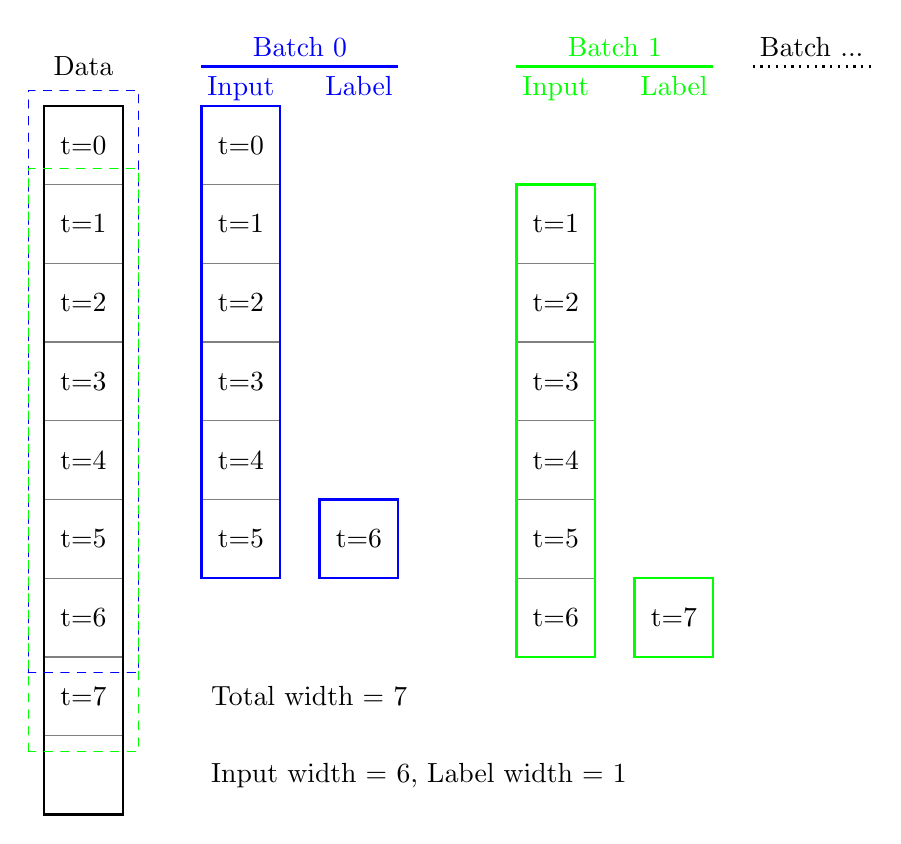
\begin{tikzpicture}

\draw[step=1cm,gray, thin] (1,1) grid (2,10);

\draw[thick, black] (1,1) rectangle (2,10);

\draw[thin, blue, line cap=round, dashed] (0.8,2.8) rectangle (2.2,10.2);

\draw[thin, green, line cap=round, dashed] (0.8,1.8) rectangle (2.2,9.2);

\foreach \x in {7,...,0} 
  \node at (1.5, 9.5 - \x ) {t=\x};

\node at (1.5,10.5) {Data};

\draw[thick, blue] (3,10.5) -- (5.5,10.5)
  node[pos=0.5,above] {Batch 0}
  node[pos=0.2,below] {Input}
  node[pos=0.8,below] {Label};
\draw[step=1cm, gray, thin] (3,4) grid (4,10);
\draw[thick, blue] (3,4) rectangle (4,10);
\draw[thick, blue] (4.5,4) rectangle (5.5,5);
\node at (5, 4.5 ) {t=6};
\foreach \x in {5,...,0} 
  \node at (3.5, 9.5 - \x ) {t=\x};


\draw[thick, green] (7,10.5) -- (9.5,10.5)
  node[pos=0.5,above] {Batch 1}
  node[pos=0.2,below] {Input}
  node[pos=0.8,below] {Label};
\draw[step=1cm, gray, thin] (7,3) grid (8,9);
\draw[thick, green] (7,3) rectangle (8,9);
\draw[thick, green] (8.5,3) rectangle (9.5,4);
\node at (9, 3.5 ) {t=7};
\foreach \x in {6,...,1} 
  \node at (7.5, 9.5 - \x ) {t=\x};

\draw[thick, black, dotted] (10,10.5) -- (11.5,10.5)
    node[pos=0.5,above] {Batch ...};

    \node[right] at (3,2.5) {Total width = 7};
    \node[right] at (3,1.5) {Input width = 6, Label width = 1};
  
\end{tikzpicture}


\end{document}

